\documentclass[conference]{IEEEtran}
\IEEEoverridecommandlockouts
% The preceding line is only needed to identify funding in the first footnote. If that is unneeded, please comment it out.
\usepackage{cite}
\usepackage{amsmath,amssymb,amsfonts}
\usepackage{algorithmic}
\usepackage[dvipdfmx]{graphicx}
\usepackage{textcomp}
\usepackage[dvipdfmx]{xcolor}
\def\BibTeX{{\rm B\kern-.05em{\sc i\kern-.025em b}\kern-.08em
    T\kern-.1667em\lower.7ex\hbox{E}\kern-.125emX}}
\begin{document}

\title{Magnet or Sticky? A Stack Overflow Tag-by-Tag Typology\\
% {\footnotesize \textsuperscript{*}Note: Sub-titles are not captured in Xplore and
% should not be used}
\thanks{Identify applicable funding agency here. If none, delete this.}
}

% \author{\IEEEauthorblockN{1\textsuperscript{st} Given Name Surname}
% \IEEEauthorblockA{\textit{dept. name of organization (of Aff.)} \\
% \textit{name of organization (of Aff.)}\\
% City, Country \\
% email address}
% \and
% \IEEEauthorblockN{2\textsuperscript{nd} Given Name Surname}
% \IEEEauthorblockA{\textit{dept. name of organization (of Aff.)} \\
% \textit{name of organization (of Aff.)}\\
% City, Country \\
% email address}
% \and
% \IEEEauthorblockN{3\textsuperscript{rd} Given Name Surname}
% \IEEEauthorblockA{\textit{dept. name of organization (of Aff.)} \\
% \textit{name of organization (of Aff.)}\\
% City, Country \\
% email address}
% \and
% \IEEEauthorblockN{4\textsuperscript{th} Given Name Surname}
% \IEEEauthorblockA{\textit{dept. name of organization (of Aff.)} \\
% \textit{name of organization (of Aff.)}\\
% City, Country \\
% email address}
% \and
% \IEEEauthorblockN{5\textsuperscript{th} Given Name Surname}
% \IEEEauthorblockA{\textit{dept. name of organization (of Aff.)} \\
% \textit{name of organization (of Aff.)}\\
% City, Country \\
% email address}
% \and
% \IEEEauthorblockN{6\textsuperscript{th} Given Name Surname}
% \IEEEauthorblockA{\textit{dept. name of organization (of Aff.)} \\
% \textit{name of organization (of Aff.)}\\
% City, Country \\
% email address}
% }

\maketitle

\begin{abstract}
Stack Overflow (SO) is one of the most popular question and answer website among engineers. There are many tags in Stack Overflow, and with the tag, you can find the questions of your interest smoothly. Many questions and answers are received every day for Stack Overflow. We explored how their interest shifed from how they use tags. We classified tags into four types: (1) attractive, (2) stagnant, (3) fluctuating, and (4) terminal based on magnet values and sticky values. Analysis of stack overflow revealed that: 
(1) There were some historical events when there were characteristics in the transition of magnet value and sticky value.
(2) Since the total number of users of stack overflow increases year by year, the graphs of magnet value and sticky value fall to the right, but if they are normalized, the sticky value of the tag is relatively outputted and a new viewpoint is revealed.
(3) In quadrant transitions, tags often remain in the same quadrant.
\end{abstract}

% \begin{IEEEkeywords}
% component, formatting, style, styling, insert 
% \end{IEEEkeywords}

\section{Introduction}
Pew Research Center, an organization that studies problems in the United States and the world, investigated society and population using US tax survey data.  States that have a high percentage of people migrating from the outside are defined as \emph{magnet states} and states where the high proportion of the population who continues to live in the same state since birth are defined as \emph{sticky states}. For example, 86\% of Nevada's population migrated from other states so Nevada state is quite "magnet". Through such a survey, you can find the tendency how American citizens move.

\smallskip
For many engineers, it is important to know the changes in the interests of other engineers. To make a project better, excellent engineers need to be interested in the project over the long term. According to the definition of magnet and sticky to be defined later, we classified tags used for stack overflow into magnet tags and sticky tags. In addition we define attagnifying strong magnetic and strong sticky \emph{attractive}, strong magnet weak sticky \emph{stagnant}, weak magnet strong sticky \emph{fluctuating}, weak magnet defines a weak sticky \emph{terminal}. By classifying like this, we analyzed what we know from the popularity of tags. We examined tags' magnets and sticky values by classifying them as tags \emph{programming language}, \emph{framework}, \emph{environment}, \emph{OS} and researching theme by theme. We also compared the news and history of the IT industry, if there are characteristic changes in magnet values and sticky values, we examined why it was like that. We addressed the following two issues:
\par
\smallskip
\textbf{(RQ1) What are typical values of magnet and sticky in Stack Overflow?}\par
In many cases, the sticky value tended to be higher than the magnet value. In addition, the decrease rate was higher for the magnet value than for the sticky value. Among them, the sticky value of swift and go rose.

\textbf{(RQ2) How do magnet and sticky values change over the time?}\par
In our research we can identify which tags are obsolete. When the tags move quadrant, we find that something happen.

\section{defination of magnet and sticky}
Measuring Contributor Retention and Attraction in Questions of Stack Cverflow

This section describes how we measure the appeal and adhesion of users on different topics on Stack Overflow.In this study, we use the Magnet and Sticky metrics defined by the Pew Research Center [26] for illustrating the migratory trends of citizens in the United States.

The Pew Research Center report1 defines magnet states as those states where a large proportion of adults who live there have moved from another state. Thus, the magnet metric for a state is the proportion of adult residents of a state who were not born in the state. Furthermore, the report also defines sticky states as those states where a large proportion of adults who were born there continue to live there. Thus, the sticky metric for a state is the proportion of adult residents who were born in the state

*These definitions are sound for a study of populations, where a single adult can only occupy one state at a time.However, the definition cannot be applied directly to the topics discussed by the users of Stack Overflow where **a user can ask or answer questions in several topics at the same time. *Therefore, we expand original definition to apply to topics in Stack Overflow as follows:

\medskip
\subsection*{\textit{\textbf{Topics discussed in Stack Overflow}}}

Questions in Stack Overflow are composed of the content of the question, answers to the question and comments ,which are call Posts in the database of SOtenent. Each question have one or more tags that separate the question into different topics. Simultaneously, Posts in a qustion have their own creater (For the content of question, one is the questioner, and for the answer, one is the respondent.)who is participant of the topics of the question.we also define the acitivity of asking or answering questions in some topic as disscussion of the topic For example, a classical questions in Stack overflow has three tags like <java>, apache and linux which is asked by user A and answered by user B, and C, so A ,B and C are participants of topic java apache and linux, by the way , We will discuss the participation of specific topics in several major categories(e.g C++ and program language), so the three topics java apache and linux are also belong to major categories Program language , Framework and OS.

\subsection*{Magnet}
Magnets are those that attract a large proportion of new users. Thus, we calculate the magnetism of a topic as the proportion of users who ask or answer during the time period under research to all new users who resigster their account at the year.

\subsection*{Sticky}
Sticky topics are those where a large proportion of the users will keep participating in discussion in the time period under research and the following. Thus, we calculate the stickiness of a topic as the proportion of the users who discuss within the topic in the time period under research to who have also discuss in the following time period.

\begin{figure}[t]
 \centering
 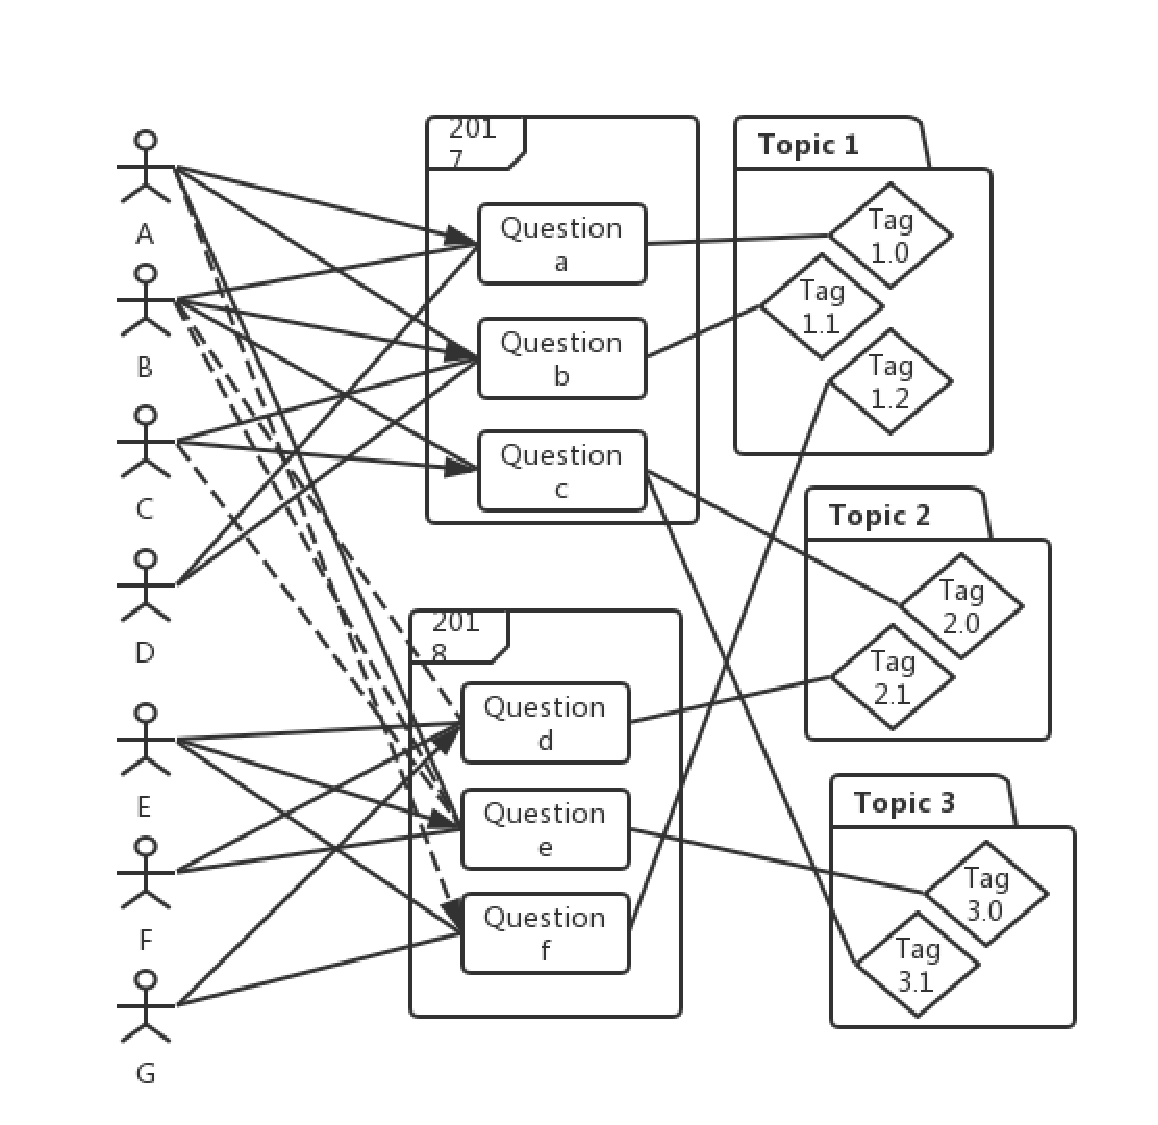
\includegraphics[width=.9\hsize]{img/examplegraph1.eps}  
 \caption{example graph} 
 \label{fig:example1} 
\end{figure}


Let us take the survey of magnet and sticky of some topics belong to a major category as a exmaple . There are 6 questions (a,b, c, d, e, f) and 7 users (A, B, C, D, E, F, G), the Last Activity Date of question a, b, c is during 2017 and question d ,e, f is during 2018. the register date of user A, B, C, D is during 2017 and the register date of user E, F, G is during 2018.

Questions have different tags. We merge tags belonging to the same topic into one topic ,for example tag "python-2.7" and tag "python-3.6" are merged into topic "python". so we get 3 topics in this case.

To calculate the magnet metric, we observe that there are four new users who register his/her account in 2017 (A, B, C and D), and all of them discuss in topic 1, while two users (BC) discuss in topic 2 and two users participate in the disccusion of topic 3. In this case, Magnet value of topic 1 in 2017 is 4/4 , topic 2 is 2/4 and topic is 2/4.

To calculate the sticky metric, on topic 1, there are three users participate in the discussion in 2017 (A, B and C) but only one of them also participate in the discussion in 2018 (A). Hence, the sticky value of project 1 is 1/4 . on topic 2, there are 2 users participate in the discussion in 2017 (B and C) but only one of them also participate in the discussion in 2018 (B). Even though new users E F G participate in the discussion in 2018, we still calculate the value of sticky as 1/2 .For the same reason, the sticky of topic 3 is 2/2 in 2018


\section{STUDY RESULTS} %paragraph4
We got research results and faced two questions against these results. We discuss the questions based on the results.

\textbf{(RQ1) What are typical values of magnet and sticky in OSS?}

We have calculated magnet and sticky values as defined in section 2. And we plotted the magnet value on the vertical axis and the sticky value on the horizontal axis. We classified the plotted points into 4 quadrants.

\smallskip
\textbf{Attractive:} Tag with high magnet and sticky value. By knowing attractive tags we can find out what the engineers are interested in.\\
\textbf{Fluctuating:} Tagwith high magnet and low sticky value. This tag attracts people but it is short-term. Excellent engineers will not continue to be interested.\\
\textbf{Stagnant:} Tag with low magnet and high sticky value. These tags are difficult to attract new users, but maintain existing users.\\
\textbf{Terminal:} Tag with Low magnet and low sticky value. This tag can neither attract new users' engineers nor keep them interested.\\
\smallskip
In this paper, the median of magnet and sticky values for each year is used for the threshold of the quadrant because the median value is not much affected by outliers. As we showed the sticky value definition in section 2, the sticky value depends on the number of tag users in that year and the following year. So in order to answer RQ1, we got 9 years' worth of sticky value from the information on the number of tag users from 2009 to 2018. The sticky value must depend on the number of new tag users but if the number of new tag users in the target year is too low, the sticky value will be too small. Therefore, in order to remove noise, we decided thresholds for each topic, and we set them all below zero. 
\medskip

\begin{figure}[t]
 \centering
 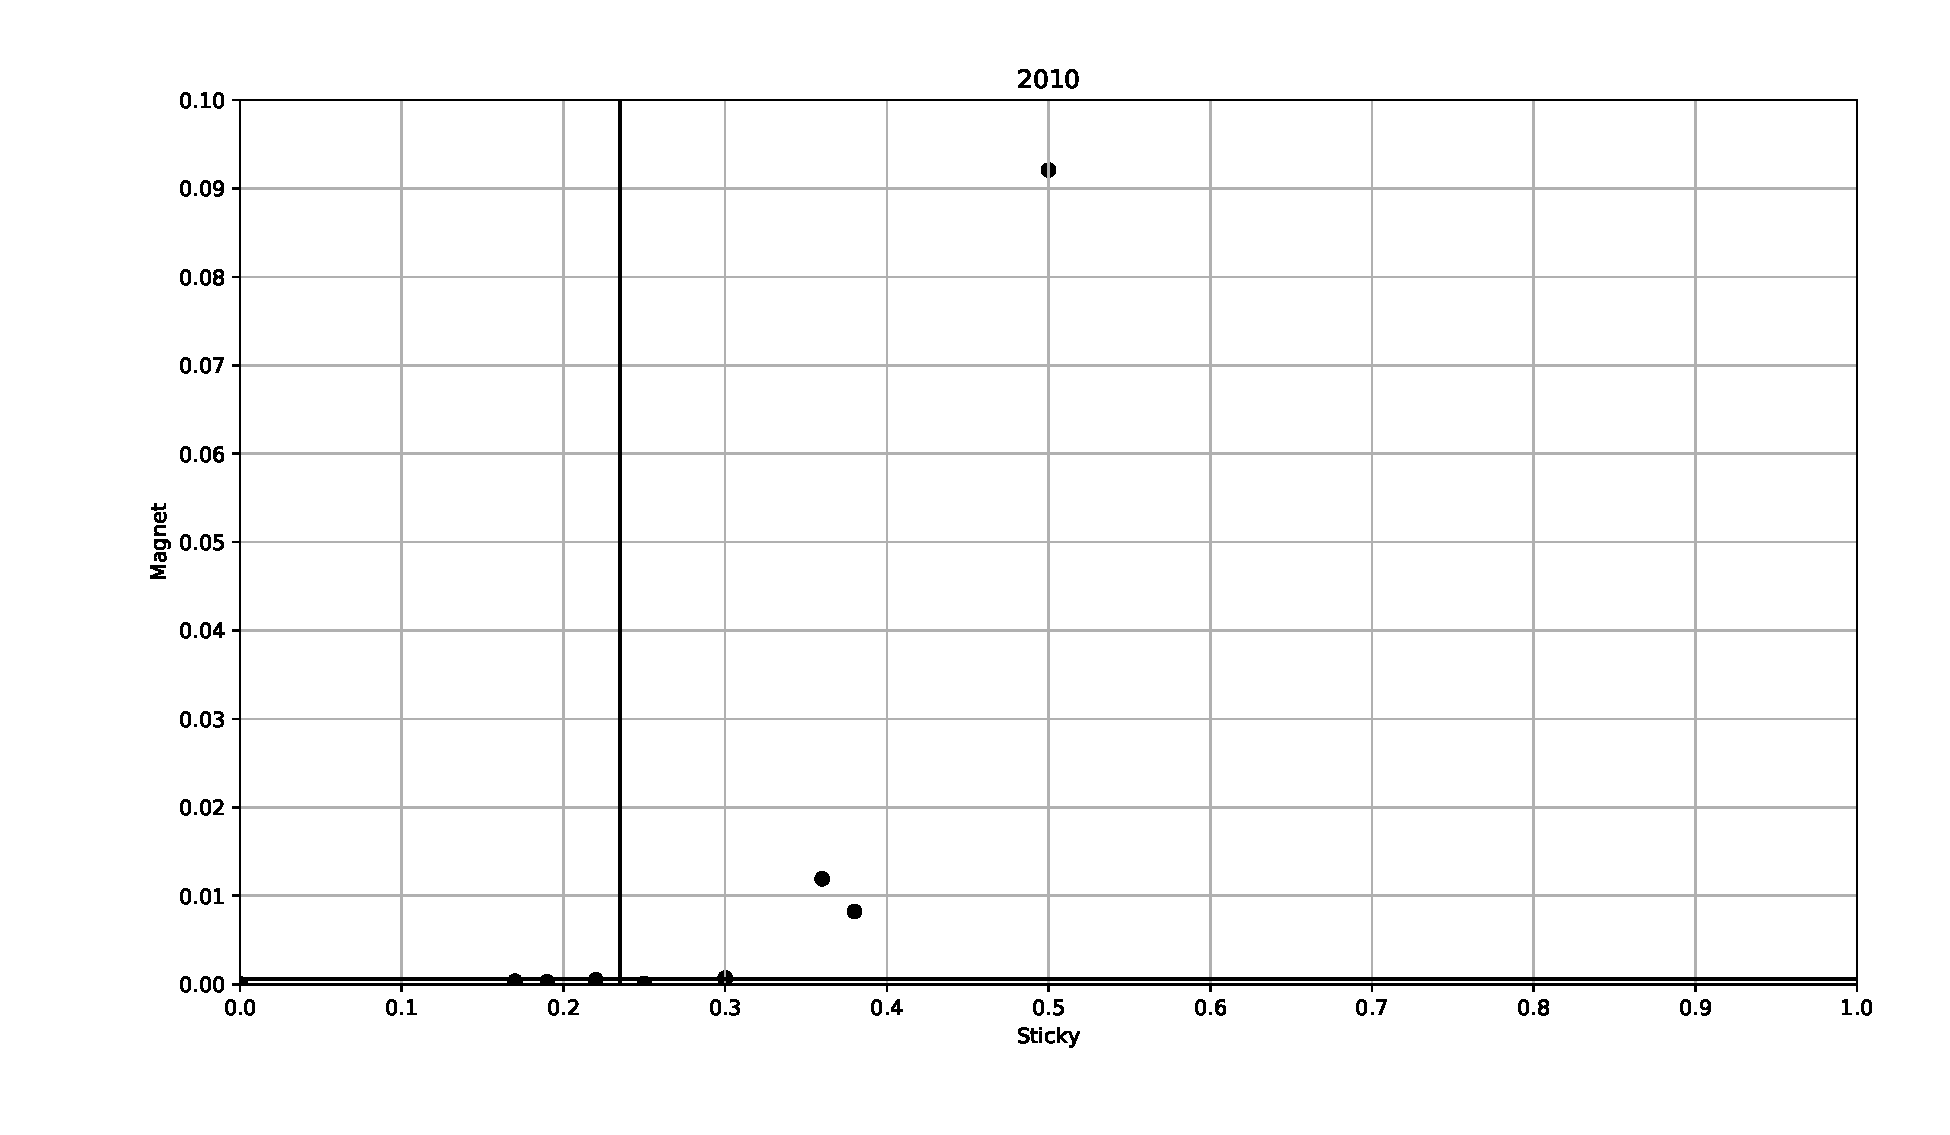
\includegraphics[width=.9\hsize]{img/plot_frame_2010.eps}  
 \caption{plotframe2010} 
 \label{fig:plotframe2010} 
\end{figure}

\textbf{Quantitive results:}
Figure\ref{fig:plotframe2010} is the magnet vs sticky value quadrant plots of the 2010 framework tag. It shows that there are points with extreme magnet and sticky values. The attractive tags are in the first quadrant, the stagnant tags are in the second quadrant, the fluctuating tags are in the third quadrant, and the terminal tags are in the fourth quadrant. From the figure, it can be seen that the value of magnet is considerably lower than the value of sticky. In other words, tags used for stack overflow are generally sticky instead of magnet. This also applies to the investigation of the Pew Research Center mentioned earlier. Engineers tend to continue to develop using the tags of the same content so that those who continue living on the same land rather than citizens living in the same place will be able to spend more time. 

\textbf{Manual analysis:}
From the figure ??? .net is high sticky and magnet value. It can be said that it is very good to be a high magnet and sticky value. The .NET Framework was published by Microsoft in November 2006. This is the foundation system for building applications on the network.  Microsoft .NET aims to connect all digital information equipment to the network, as well as electronic equipment such as personal computers, servers, mobile phones, smart phones, home appliances, etc. and to be accessible anytime via the Internet. It is the .NET Framework that framed it using the .NET environment. On this framework, it is possible to develop and execute software supporting the .NET environment. The reason why the .NET magnet value is high is beginner engineers can develop somewhat advanced software. The reason why .NET's sticky value is high is its convenience.
\medskip
 
% \usepackage{ascmac}

% \begin{document}
%   \begin{screen}
 \emph{Sticky is a more general attribute than magnet. Tags with high magnet value are easy to use even for beginners. Especially magnet tags like .NET are relatively easy to use, so it is widely used for beginners and others. Machine learning gradually became fashionable around 2015 and as it is now, sticky values such as machine learning library like torch are high.}
%   \end{screen}
% \end{document}
\medskip


\begin{figure}[t]
 \centering
 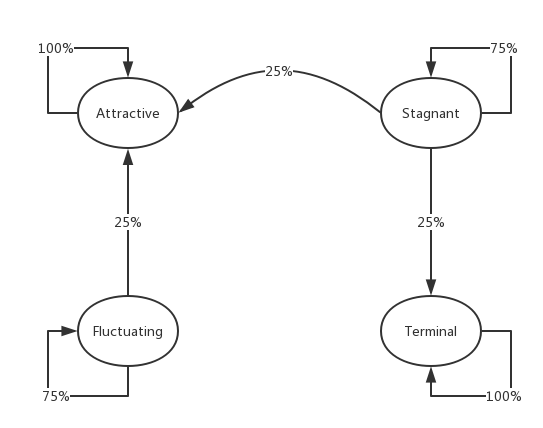
\includegraphics[width=.9\hsize]{img/Lang2017.eps}  
 \caption{The Transition of Programing Language in 2017} 
 \label{fig:envtrans2018} 
\end{figure}

\textbf{(RQ2) How do magnet and sticky values change over time?} \\
\textbf{Approach:}
We investigated how the tags move with time over the quadrants of Figure\ref{envtrans2018}. 
Quantitative results:
Figure \ref{envtrans2018} indicates the quadrant transition likelihood using the state transition diagram. The values on the arrows indicate the possibility of transition from each quadrant to the quadrant. For example, Δ indicates that the transition from Stagnant to Attractive is 33\%. We use * to represent years with tag when users were less than 100 people.
As you can see from the figure, the tags are moving only from Fluctuating to Terminal. Tags with popular fluctuations are sometimes no longer used by anyone. Also, you can see that all tags often stay in the same quadrant. Attractive tags may settle to Stagnant and Stagnant tags become popular and sometimes become Attractive tags. Manual analysis:
Figure A shows the transition of the quadrant of each tag. From this figure, we learn how the tags transition the quadrants.
From Figure A, it turns out that the programming language often stays in the same quadrant. Also, between Attractive and Stagnant, the transition frequently occurs, indicating that the transition between Terminal and Flactuating changes well.\\

\medskip
\emph{As a result of investigating from 2009 to 2018, in the programming language, the average transition from Attractive to Attractive was 91.5\%, the transition from Fluctuating to Fluctuating was 77.8\%, the change from Stagnant to Stagnant was 80.6\%, and the change from Terminal to Terminal was 87.2\%.  In the programming language, it turned out that the classification of tags was difficult to change.}
\medskip



\section{Conclusion}

Whether it's a programming language or a program framework or an operating system, keeping the community alive and attracting more people to participate in discussions is critical to its development.Especially on the stack overflow, the world's largest program Q\&A platform, having more questions and answers on a topic means that customers of the product are more likely to solve their own problems, which is even more tedious than that developers rack their brains to write a lengthy development document or Q\&A This paper applied the magnet and sticky population concepts to a set of topics in Stack Overflow. We find that:

1. The number of topics that people participate in is exploding with the development and popularity of computer technology.Even the most popular themes can't attract the high percentage of people involved in the discussion like what they did ten years ago.\\


2. Under their respective major categories, the most popular topics are still very popular after ten years, and only a small number of languages or frameworks can stand out and become one of the most popular topics.\\


3. This research can provide some reference for enterprises to choose their own main technology stack, and can also be used as a reference for computer science students to learn new technologies, because it (1)predicts the trend of computer technology in the next few years, (2)points out which technologies are easier to access and the questions can be easier to get answers to.\\



\section{ACKNOWLEDGEMENTS}


% \begin{table}[htbp]
% \caption{Table Type Styles}
% \begin{center}
% \begin{tabular}{|c|c|c|c|}
% \hline
% \textbf{Table}&\multicolumn{3}{|c|}{\textbf{Table Column Head}} \\
% \cline{2-4} 
% \textbf{Head} & \textbf{\textit{Table column subhead}}& \textbf{\textit{Subhead}}& \textbf{\textit{Subhead}} \\
% \hline
% copy& More table copy$^{\mathrm{a}}$& &  \\
% \hline
% \multicolumn{4}{l}{$^{\mathrm{a}}$Sample of a Table footnote.}
% \end{tabular}
% \label{tab1}
% \end{center}
% \end{table}

% \begin{figure}[htbp]
% \centerline{
\includegraphics{fig1.png}}
% \caption{Example of a figure caption.}
% \label{fig}
% \end{figure}

% Figure Labels: Use 8 point Times New Roman for Figure labels. Use words 
% rather than symbols or abbreviations when writing Figure axis labels to 
% avoid confusing the reader. As an example, write the quantity 
% ``Magnetization'', or ``Magnetization, M'', not just ``M''. If including 
% units in the label, present them within parentheses. Do not label axes only 
% with units. In the example, write ``Magnetization (A/m)'' or ``Magnetization 
% \{A[m(1)]\}'', not just ``A/m''. Do not label axes with a ratio of 
% quantities and units. For example, write ``Temperature (K)'', not 
% ``Temperature/K''.

% \section*{Acknowledgment}

% The preferred spelling of the word ``acknowledgment'' in America is without 
% an ``e'' after the ``g''. Avoid the stilted expression ``one of us (R. B. 
% G.) thanks $\ldots$''. Instead, try ``R. B. G. thanks$\ldots$''. Put sponsor 
% acknowledgments in the unnumbered footnote on the first page.

% \section*{References}

% Please number citations consecutively within brackets \cite{b1}. The 
% sentence punctuation follows the bracket \cite{b2}. Refer simply to the reference 
% number, as in \cite{b3}---do not use ``Ref. \cite{b3}'' or ``reference \cite{b3}'' except at 
% the beginning of a sentence: ``Reference \cite{b3} was the first $\ldots$''

% Number footnotes separately in superscripts. Place the actual footnote at 
% the bottom of the column in which it was cited. Do not put footnotes in the 
% abstract or reference list. Use letters for table footnotes.

% Unless there are six authors or more give all authors' names; do not use 
% ``et al.''. Papers that have not been published, even if they have been 
% submitted for publication, should be cited as ``unpublished'' \cite{b4}. Papers 
% that have been accepted for publication should be cited as ``in press'' \cite{b5}. 
% Capitalize only the first word in a paper title, except for proper nouns and 
% element symbols.

% For papers published in translation journals, please give the English 
% citation first, followed by the original foreign-language citation \cite{b6}.

% \begin{thebibliography}{00}
% \bibitem{b1} G. Eason, B. Noble, and I. N. Sneddon, ``On certain integrals of Lipschitz-Hankel type involving products of Bessel functions,'' Phil. Trans. Roy. Soc. London, vol. A247, pp. 529--551, April 1955.
% \bibitem{b2} J. Clerk Maxwell, A Treatise on Electricity and Magnetism, 3rd ed., vol. 2. Oxford: Clarendon, 1892, pp.68--73.
% \bibitem{b3} I. S. Jacobs and C. P. Bean, ``Fine particles, thin films and exchange anisotropy,'' in Magnetism, vol. III, G. T. Rado and H. Suhl, Eds. New York: Academic, 1963, pp. 271--350.
% \bibitem{b4} K. Elissa, ``Title of paper if known,'' unpublished.
% \bibitem{b5} R. Nicole, ``Title of paper with only first word capitalized,'' J. Name Stand. Abbrev., in press.
% \bibitem{b6} Y. Yorozu, M. Hirano, K. Oka, and Y. Tagawa, ``Electron spectroscopy studies on magneto-optical media and plastic substrate interface,'' IEEE Transl. J. Magn. Japan, vol. 2, pp. 740--741, August 1987 [Digests 9th Annual Conf. Magnetics Japan, p. 301, 1982].
% \bibitem{b7} M. Young, The Technical Writer's Handbook. Mill Valley, CA: University Science, 1989.
% \end{thebibliography}
% \vspace{12pt}
% \color{red}
% IEEE conference templates contain guidance text for composing and formatting conference papers. Please ensure that all template text is removed from your conference paper prior to submission to the conference. Failure to remove the template text from your paper may result in your paper not being published.

\end{document}
